\documentclass[12pt,a4paper]{article}

\usepackage[margin=2.3cm]{geometry}
\usepackage[T1]{fontenc}
\usepackage{amsmath,amssymb}
\usepackage{bbm}
\usepackage{graphicx}
\usepackage{booktabs}
\usepackage{parskip}

\setcounter{secnumdepth}{2}

\title{Extending Active Recommendation for Email Outreach Dynamics\\[4pt]
\large Refinements to a SAE + Thompson Sampling Bandit}
\author{Tymofii Ivanov}
\date{\today}

\begin{document}

\maketitle

\section{Overview}
\large
\begin{itemize}
  \item \textbf{Problem:} cold-start email campaigns --- new templates have no interaction history
  \item \textbf{Baseline:} SAE-based collaborative filtering + Thompson Sampling bandit over recipients
  \item \textbf{This document:} recaps the baseline, presents 9 refinements, and compares results
\end{itemize}
\normalsize

\clearpage
\section{Baseline Model}
\large
Interaction matrix $X \in \{0,1\}^{n \times m}$, $X_{i,j}=1$ iff recipient $j$ opened template $i$.

\[
  \min_{E,D} \; \ell\big(X,\, \sigma(X B_{E,D})\big), \qquad
  B_{E,D} = ED^\top - \mathrm{diag}\big([E\odot D]\mathbf{1}\big)
\]
\[
  \Sigma = \sigma(B_{E,D}) \quad \Rightarrow \quad
  \Sigma_{i,j} = P(\,j \text{ opens} \mid i \text{ already opened}\,)
\]

Each recipient $j$ is scored as:
\[
  s_j(t) = \alpha \cdot \phi_j p_j + (1-\alpha)\cdot f_j(t)
\]
\begin{itemize}
  \item $\phi_j$ --- historic open rate of recipient $j$
  \item $p_j$ --- influence of $j$ on other recipients
  \item $f_j(t)$ --- confidence $j$ opens, given current state
\end{itemize}
\[
  \alpha_j(t) = G\, s_j(t), \qquad \beta_j(t) = G\big(1-s_j(t)\big)
\]
\normalsize

\clearpage
\section{Linear Alpha Scheduling}
\large
\textbf{Problem:} a fixed $\alpha$ cannot shift from exploration to exploitation as the campaign progresses.

\[
  \alpha(\mu) = l(1-\mu) + r\mu, \qquad \mu = \tfrac{N(t)}{N}
\]

\textbf{Result} ($l=0.1$, $r=0.05$): \quad
R@5/15/25/35\% = 0.383 / 0.823 / 0.927 / 0.960 \quad AUC $= 0.894$
\normalsize

\begin{center}
  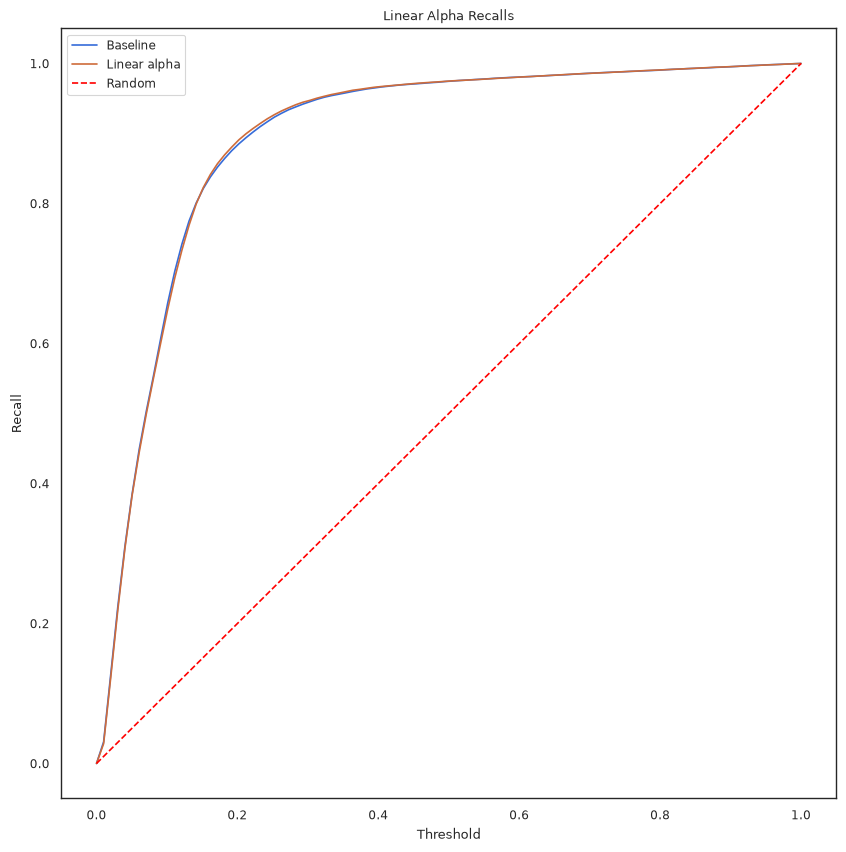
\includegraphics[width=0.6\textwidth]{images/linear_alpha_recalls_0_1.png}
\end{center}

\clearpage
\section{Geometric Alpha Scheduling}
\large
\textbf{Problem:} same motivation as linear scheduling; a log-linear decay may fit the explore/exploit shift better.

\[
  \alpha(\mu) = l^{(1-\mu)} \, r^{\mu}
\]

\textbf{Result} ($l=0.3$, $r=0.05$): \quad
R@5/15/25/35\% = 0.377 / 0.823 / 0.927 / 0.959 \quad AUC $= 0.894$
\normalsize

\begin{center}
  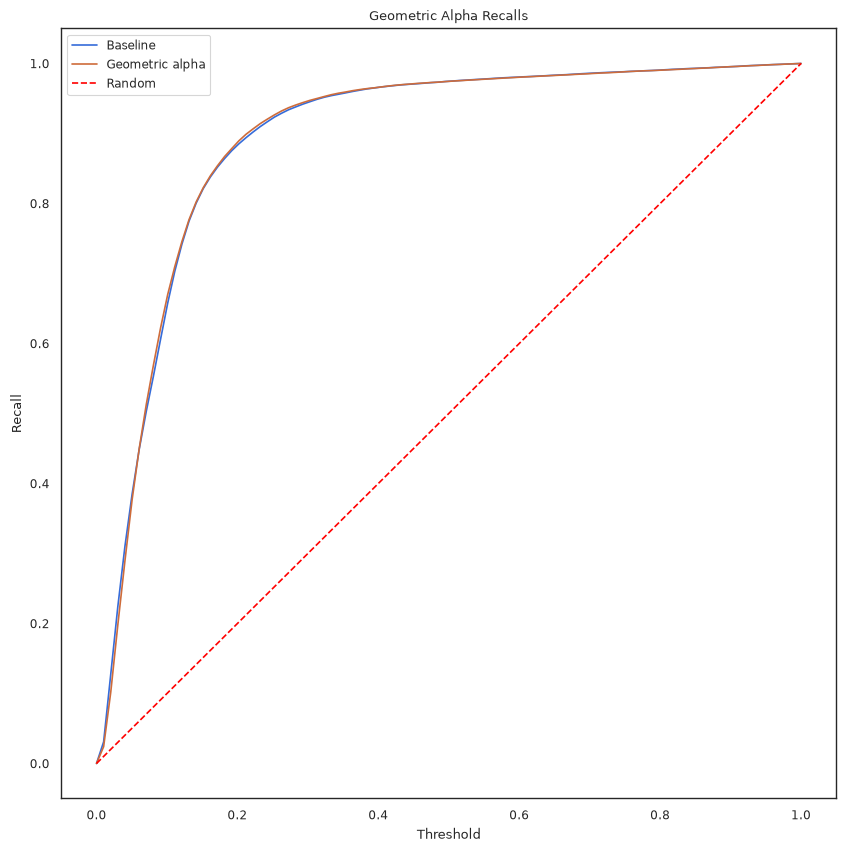
\includegraphics[width=0.6\textwidth]{images/geometric_alpha_recalls_0_1.png}
\end{center}

\clearpage
\section{Confidence-Based Alpha Scheduling}
\large
\textbf{Problem:} trust in $f_j(t)$ should grow as more opens are observed, not just as time passes.

\[
  \alpha(\tilde o) = \frac{\kappa}{\tilde o + \kappa}, \qquad \tilde o = \tfrac{o(t)}{m}
\]

\textbf{Result} ($\kappa=0.003$): \quad
R@5/15/25/35\% = 0.341 / 0.818 / 0.926 / 0.960 \quad AUC $= 0.891$
\normalsize

\begin{center}
  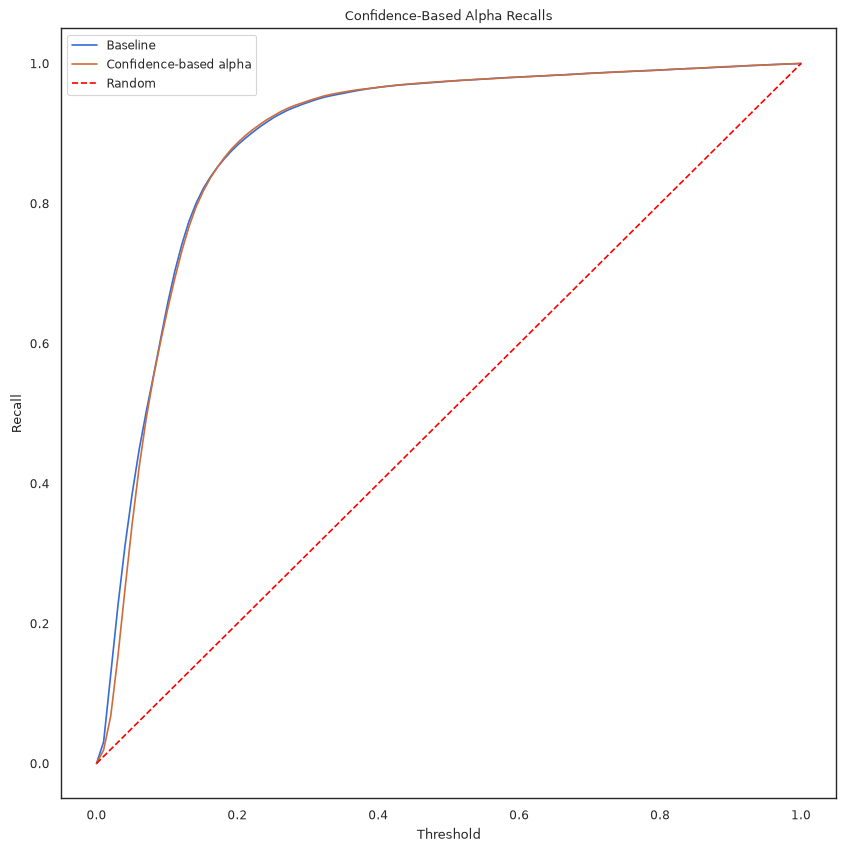
\includegraphics[width=0.6\textwidth]{images/confidence_based_alpha_recalls_0_1.png}
\end{center}

\clearpage
\section{Recency-Weighted Historical Engagement}
\large
\textbf{Problem:} $\phi_j$ weights all past templates equally, ignoring behavioral drift over time.

\[
  \omega_i = 2^{-d_i/h}, \qquad
  \phi_j = \frac{\omega^\top X_{:,j}}{\sum_i \omega_i}
\]

\textbf{Result} ($h=0.3$): \quad
R@5/15/25/35\% = 0.447 / 0.837 / 0.928 / 0.960 \quad AUC $= 0.903$
\normalsize

\begin{center}
  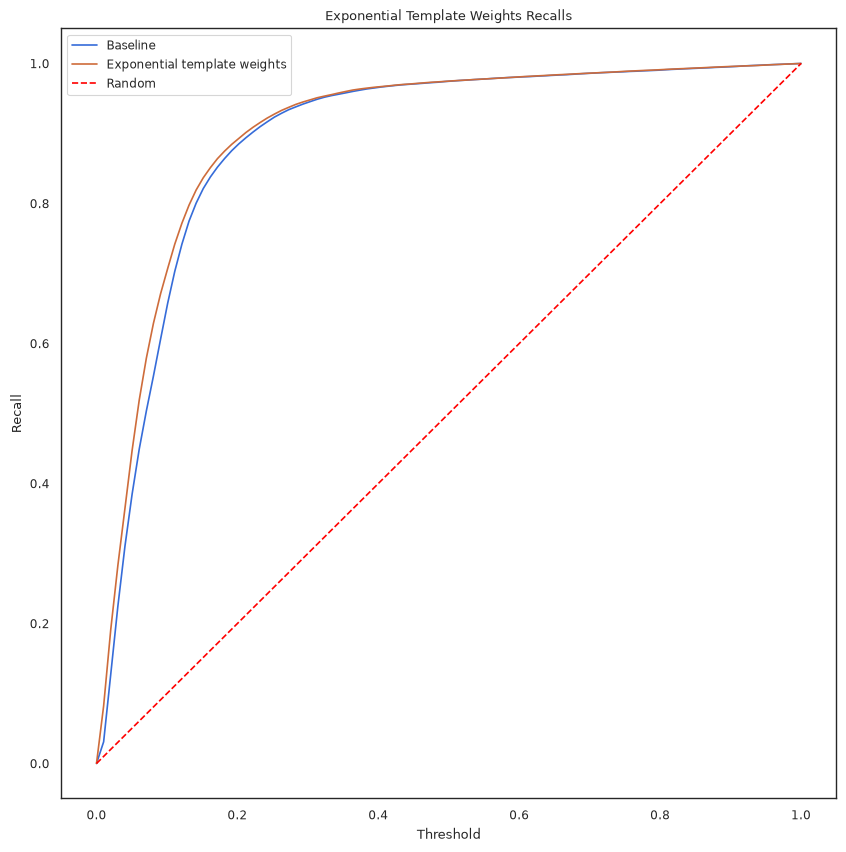
\includegraphics[width=0.6\textwidth]{images/exp_template_weight_recalls_0_1.png}
\end{center}

\clearpage
\section{Forward-Pass Definition of $f_j(t)$}
\large
\textbf{Problem:} the linear form of $f_j(t)$ cannot capture joint influence of multiple simultaneous openers.

\[
  f_j(t) = f_{SAE}\big(x(t)\big)\, e_j = \sigma\big(x(t)^\top B_{E,D}\big)\, e_j
\]

\textbf{Result:} \quad
R@5/15/25/35\% = 0.375 / 0.841 / 0.937 / 0.966 \quad AUC $= 0.901$
\normalsize

\begin{center}
  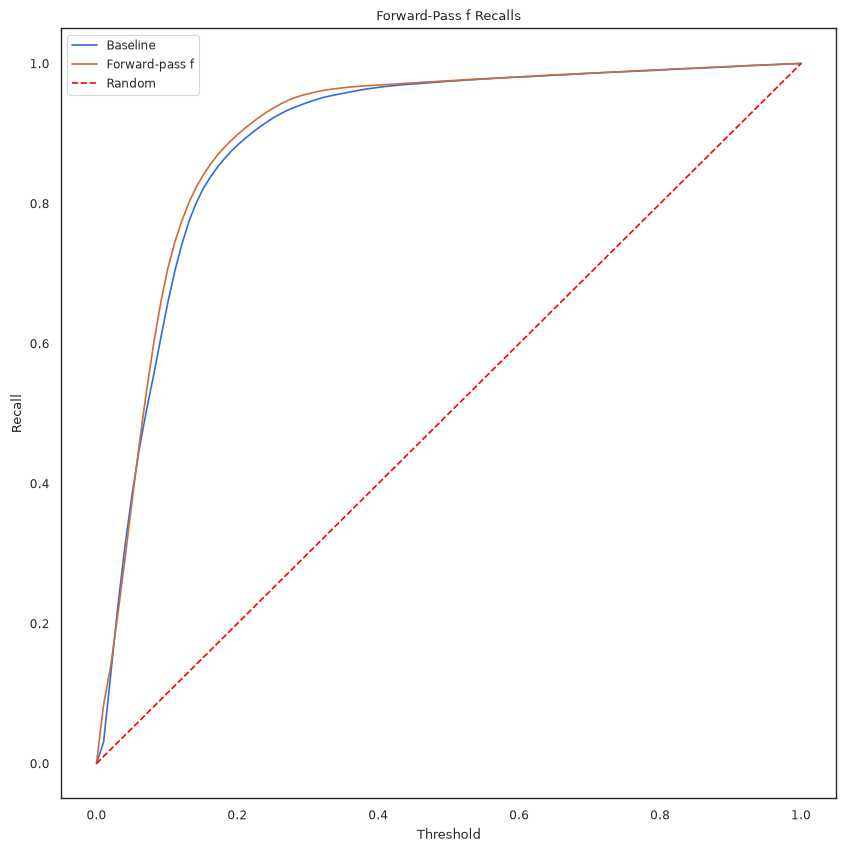
\includegraphics[width=0.6\textwidth]{images/forward_pass_f_recalls_0_1.png}
\end{center}

\clearpage
\section{Variance-Based Definition of $p_j$}
\large
\textbf{Problem:} baseline $p_j$ rewards score \emph{increase}, not the \emph{uncertainty reduction} that defines information gain.

\[
  p_j = \frac{4}{m-1}\sum_{i\ne j} \big(\Sigma_{j,i} - \bar\Sigma_{j,:}\big)^2
\]

\textbf{Result:} \quad
R@5/15/25/35\% = 0.479 / 0.837 / 0.926 / 0.960 \quad AUC $= 0.905$
\normalsize

\begin{center}
  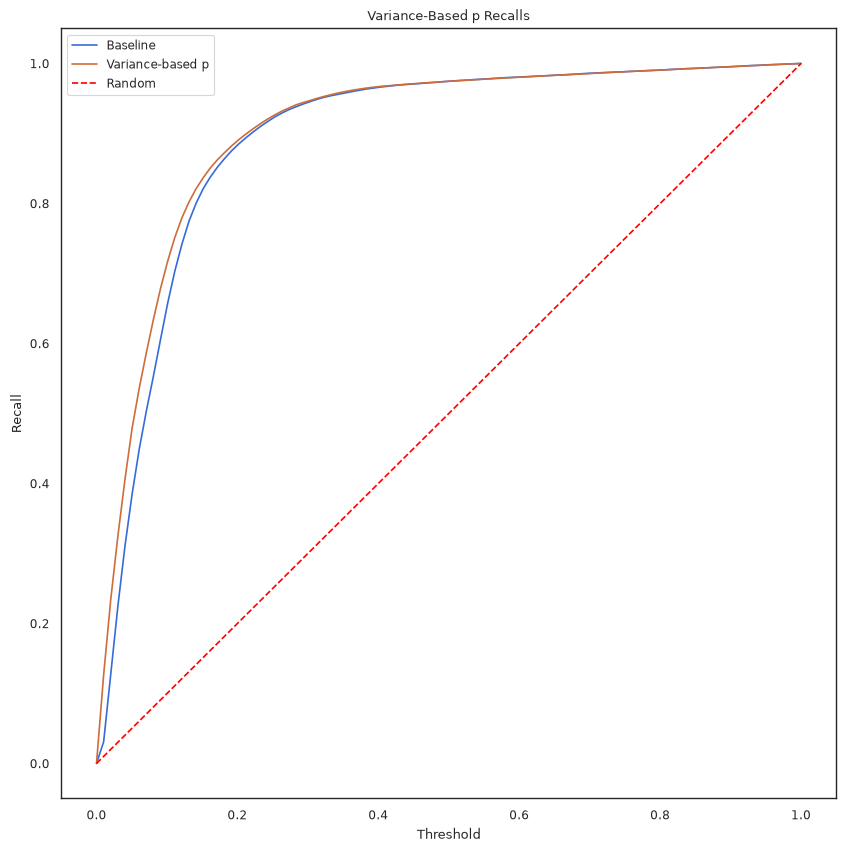
\includegraphics[width=0.6\textwidth]{images/variance_based_p_recalls_0_1.png}
\end{center}

\clearpage
\section{Multiplicative Score Decomposition}
\large
\textbf{Problem:} the baseline conflates two axes --- explore/exploit and historic/current data --- into one linear term.

\[
  s_j(t) = \pi_j(t)\, u_j(t)
\]
\[
  \pi_j(t) = \alpha(t)\phi_j + (1{-}\alpha(t))f_j(t), \qquad
  u_j(t) = \beta(t)p_j + (1{-}\beta(t))\cdot 1
\]

\textbf{Result:} \quad
R@5/15/25/35\% = 0.425 / 0.821 / 0.922 / 0.959 \quad AUC $= 0.900$
\normalsize

\begin{center}
  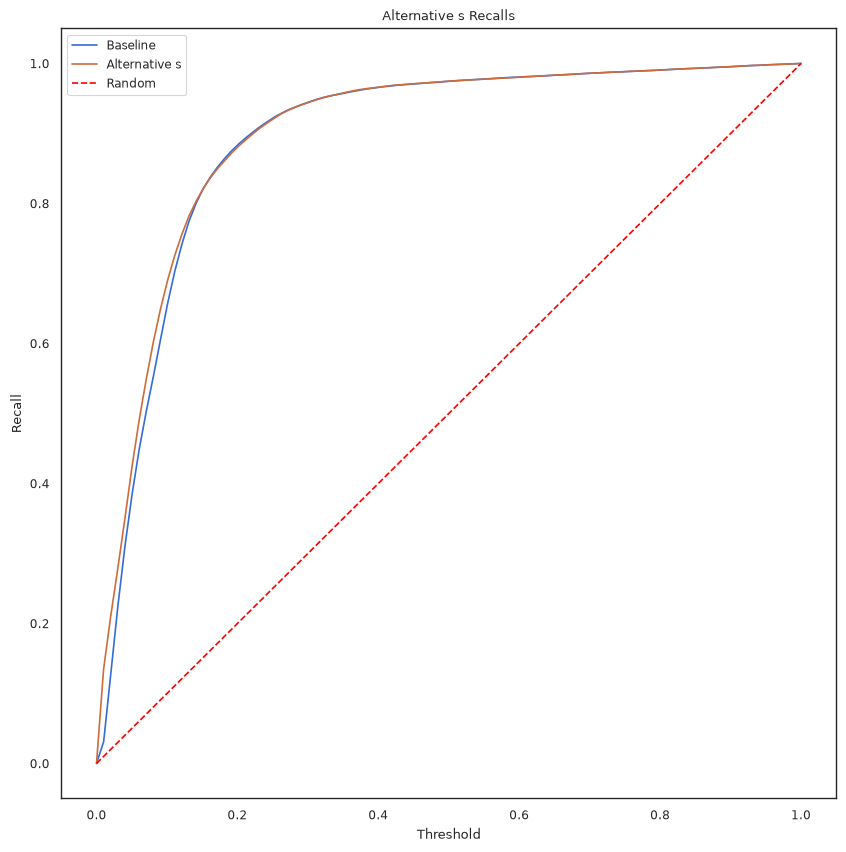
\includegraphics[width=0.55\textwidth]{images/alternative_s_recalls_0_1.png}
\end{center}

\clearpage
\section{Binary-to-TTO Model ($X \to Y$)}
\large
\textbf{Problem:} two recipients who both eventually open are treated identically by the SAE, regardless of how fast they did it --- discarding available time-to-open signal.

\[
  Y_{i,j} = 2^{-\Delta_{i,j}/h_\delta} \in [0,1], \qquad \Delta_{i,j} = \text{observed send-to-open time}
\]
\[
  \min_{E,D} \; \ell\big(Y,\, \sigma(X B_{E,D})\big)
\]

Input space stays binary ($x$); only the reconstruction target is swapped for the TTO-decayed label $Y$. Since $e_j$ is unchanged as a training-time input, $p_j$ carries over \textbf{mechanically unchanged}; $f_j(t)$ and $s_j(t)$ require no further modification to run end-to-end.

\textbf{Status:} proposed formulation, not yet benchmarked.
\normalsize

\clearpage
\section{TTO Cutoff Thresholding}
\large
\textbf{Problem:} SAE trains on fully-converged opens, but active-learning queries $x(t)$ are always incomplete.

\[
  C_{i,j} = \mathbbm{1}[\Delta_{i,j} \le \delta_c], \qquad
  \min_{E,D} \ell\big(X,\, \sigma(C B_{E,D})\big)
\]

\textbf{Result} ($\delta_c=720$): \quad
R@5/15/25/35\% = 0.390 / 0.824 / 0.924 / 0.960 \quad AUC $= 0.895$
\normalsize

\begin{center}
  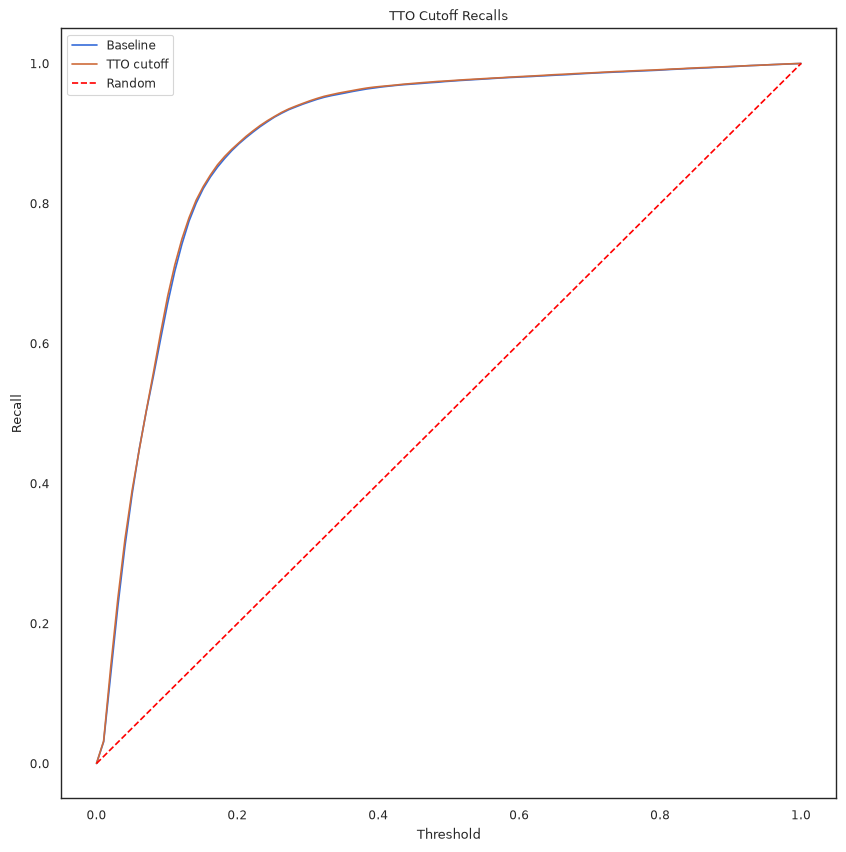
\includegraphics[width=0.6\textwidth]{images/tto_cutoff_recalls_0_1.png}
\end{center}

\clearpage
\section{Nonlinear (Deep) Autoencoder}
\large
\textbf{Problem:} the linear SAE can only capture linear recipient--recipient relationships.

\[
  \text{Enc:}\ m \to 2d \to d, \qquad \text{Dec:}\ d \to 2d \to m \qquad (\text{ReLU, denoising mask})
\]

\textbf{Result} ($d=16$): \quad
R@5/15/25/35\% = 0.400 / 0.815 / 0.936 / 0.963 \quad AUC $= 0.898$
\normalsize

\begin{center}
  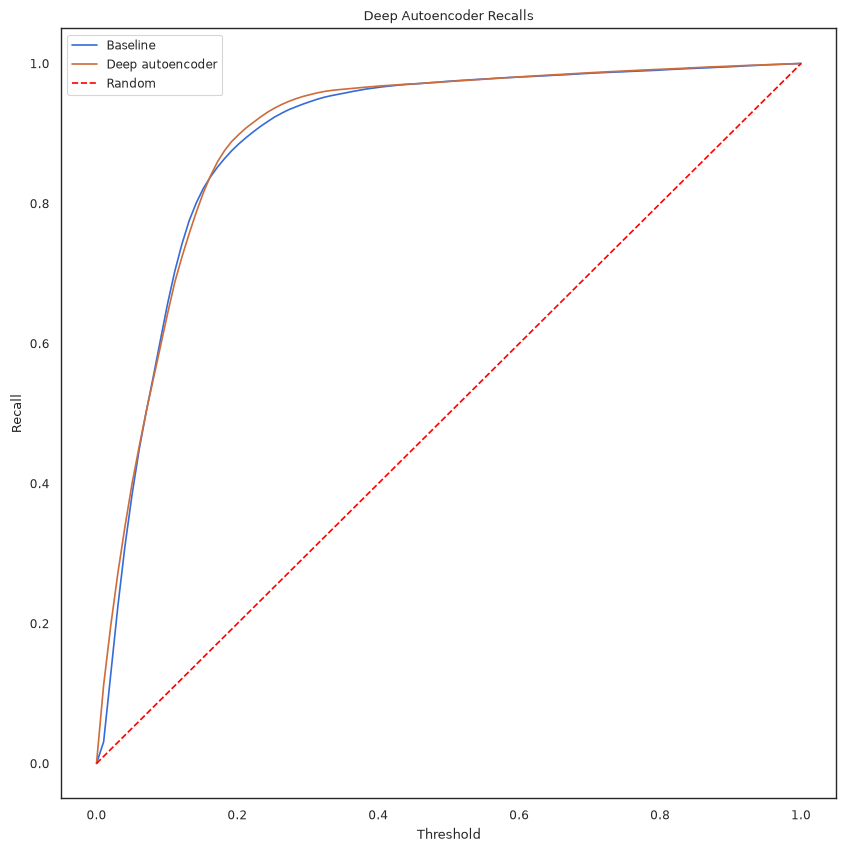
\includegraphics[width=0.6\textwidth]{images/deep_autoencoder_recalls_0_1.png}
\end{center}

\clearpage
\section{Further Refinements (Untested)}
\large
\begin{itemize}
  \item \textbf{Deep autoencoder regularization:} stronger latent-space dropout; dropout inside the encoder/decoder layers themselves, beyond the current denoising mask
  \item \textbf{Further TTO extensions:} a $Y \to Y$ model (continuous signal on the input side too, not just the target); $z(t)$ interpolation --- a partially TTO-informed query state at inference instead of binary $x(t)$
  \item \textbf{Alternative $p_j$ definitions:} clustering-based influence scores; time-dependent $p_j(t)$
  \item \textbf{Plug-and-play $s_j(t)$:} the multiplicative decomposition reuses the original primitives, so many of the above can be swapped in directly
  \item \textbf{TTO-based noise injection:} corrupt training rows using TTO-derived noise
\end{itemize}
\normalsize

\clearpage
\section{Results Summary}
\centering
\renewcommand{\arraystretch}{1.3}
\begin{tabular}{lccccc}
  \toprule
  \textbf{Model} & \textbf{R@5\%} & \textbf{R@15\%} & \textbf{R@25\%} & \textbf{R@35\%} & \textbf{AUC} \\
  \midrule
  Baseline                      & 0.385 & 0.821 & 0.923 & 0.958 & 0.894 \\
  Linear $\alpha$ schedule      & 0.383 & 0.823 & 0.927 & 0.960 & 0.894 \\
  Geometric $\alpha$ schedule   & 0.377 & 0.823 & 0.927 & 0.959 & 0.894 \\
  Confidence $\alpha$ schedule  & 0.341 & 0.818 & 0.926 & 0.960 & 0.891 \\
  Template weights              & 0.447 & 0.837 & 0.928 & 0.960 & 0.903 \\
  Forward-pass $f$              & 0.375 & \textbf{0.841} & \textbf{0.937} & \textbf{0.966} & 0.901 \\
  Variance-based $p$            & \textbf{0.479} & 0.837 & 0.926 & 0.960 & \textbf{0.905} \\
  Alternative $s$ decomposition & 0.425 & 0.821 & 0.922 & 0.959 & 0.900 \\
  TTO cutoff thresholding       & 0.390 & 0.824 & 0.924 & 0.960 & 0.895 \\
  Deep autoencoder              & 0.400 & 0.815 & 0.936 & 0.963 & 0.898 \\
  \bottomrule
\end{tabular}

\bigskip
\raggedright
\normalsize
Standard deviations omitted for space; see whitepaper for full statistics.

\end{document}